%\documentclass[letterpaper, onecolumn, 10pt]{article}
%\linespread{2.4}
\documentclass[letterpaper, twocolumn, 10pt]{article}
\usepackage{usenix}

\usepackage{multirow}
\usepackage{comment}
\usepackage{epsfig}
%\usepackage{kotex}
%\usepackage{amsmath}
\usepackage{amssymb}
\usepackage{multirow}
\usepackage{url}
\usepackage{subfig}
\usepackage{color}
\usepackage{xcolor}
\usepackage{cases}
\usepackage{graphicx}
%\usepackage{float}
\usepackage{caption}

\begin{document}

\title{
\bf PCStream: Automatic Stream Allocation Using Program Contexts}

%\numberofauthors{1}

\author{
{\rm Taejin Kim}\\
Seoul National University
\and 
{\rm Sangwook Shane Hahn}\\
Seoul National University
\and 
{\rm Jooyoung Hwang} \\
Samsung Electronics
\and 
{\rm Jongyoul Lee} \\
Samsung Electronics
\and 
{\rm Sungjin Lee}\\
DGIST
\and 
{\rm Jihong Kim} \\
Seoul National University
}

\maketitle

\thispagestyle{empty}

\subsection*{Abstract}
We propose a fully automatic stream management technique, called {\sf PCStream}, 
for multi-streamed SSDs.
{\sf PCStream} is based on our observation that data lifetimes can be reliably predicted using
write program contexts.  
By extracting program contexts during the run time,  
{\sf PCStream}  automates the data-to-stream mapping.  
When data mapped to the same
stream show large differences in their lifetimes, {\sf PCStream}
moves the long-lived data of the current stream to 
its substream during garbage collection.
Our experimental results show that {\sf PCStream} can reduce the
garbage collection overhead as much as manual stream
management techniques while no code modification is necessary.
For a RocksDB benchmark, {\sf PCStream} improved WAF by 40\% over 
the existing automatic technique.


\section{Introduction}
\label{sec:intro}
Multi-streamed SSDs provide a special mechanism,
called streams, for a host system to prevent data with different lifetimes 
from being mixed into the same block~\cite{T10, MultiStream}.
When the host system maps two data $D_1$ and $D_2$ to 
different streams $S_1$ and $S_2$, a multi-streamed SSD guarantees that 
$D_1$ and $D_2$ are placed to different blocks.   
Since streams, when properly managed, can be very effective in minimizing 
the copy cost of garbage collection, they
can significantly improve both the performance and lifetime of 
flash-based SSDs~\cite{MultiStream, FStream, AutoStream, Level}.

In order to achieve high performance on multi-streamed SSDs, data with similar 
{\it future} update times~\cite{PCHa}
should be allocated 
to the same stream, so that the copy cost of garbage collection can be minimized.
However, since it is difficult to know the future update times {\it a priori} when they are written,
stream allocation decisions are often {\it manually} made by programmers based on their expertise (or experience) 
on the application~\cite{MultiStream} or the file system~\cite{FStream}.  
Furthermore, these manual techniques assume a fixed number of 
streams (i.e., a specific SSD).   
When an SSD has a smaller number of streams, stream allocation decisions should be changed.
In this paper, our goal is to develop 
a {\it fully automatic} technique for managing streams 
which is applicable for {\it any} multi-streamed SSD
\footnote{The main difference among different multi-streamed 
SSDs is the maximum number of streams supported.  
For example, the SSD used in FStream~\cite{FStream} has 9 streams 
while the SSD used in AutoStream~\cite{AutoStream} has 16 streams.}.

To the best of our knowledge, AutoStream~\cite{AutoStream} is the only automatic 
stream management technique
without additional manual work.  
However, since AutoStream predicts data lifetimes using the update frequency 
of the logical block address (LBA), it does not work well with modern append-only workloads 
such as RocksDB~\cite{RocksDB} or Cassandra~\cite{Cassandra}.  
Unlike conventional update workloads where data written to the same LBAs 
often show a strong update locality, 
append-only workloads make it impossible to predict data lifetimes 
from the LBA characteristics (such as access frequency or access patterns).  
For example, as shown in Figure~\ref{fig:lba_lifetime}(b), 
data written to a fixed LBA range over times in RocksDB 
show widely varying data lifetimes, 
thus making it difficult to allocate streams based on LBA characteristics.

In this paper, we propose a fully automatic stream management technique, called {\sf PCStream}, 
for multi-streamed SSDs based on program contexts (PCs).
Since the key motivation behind {\sf PCStream} was 
that data lifetimes should be estimated at a higher abstraction level than LBAs, 
{\sf PCStream} employed a write program context\footnote{Since we are interested in write-related 
system calls such as write() and writev() in the Linux kernel, 
we call their related program contexts as 
{\it write program contexts.} In the rest of the paper, we use 
{\it program contexts} interchangeably with {\it write program contexts}.}  
as a main unit for managing streams.   
A program context~\cite{PC}, which represents a particular execution phase of a program, 
is known to be an effective hint in separating data with different lifetimes~\cite{PCHa}.  
(That is, the lifetime of data written by the same program context tends to be very similar.)   
{\sf PCStream} automatically maps an identified program context to a stream.  
Since program contexts can be computed during the run time, 
{\sf PCStream} does not need any manual work.   
In order to handle append-only workloads, 
{\sf PCStream} extended the definition of the data lifetime 
so that the effect of the TRIM command~\cite{10} can be accounted for. 

Although most program contexts show that their data lifetimes are 
distributed with small variances, we observed a few outliers 
whose data lifetimes have rather large variances.
In {\sf PCStream}, 
when such a PC {\it pID} is observed (which was mapped to a stream {\it sID}), 
the long-lived data of {\it pID} are moved to the substream of {\it sID}
during garbage collection.  
The substream prevents the long-lived data of the stream {\it sID} 
from being mixed with future short-lived data of the stream {\it sID}.

In order to evaluate the effectiveness of PCStream, we have implemented PCStream 
in the Linux kernel (v. 4.5) and measured write amplification factor (WAF) values 
using RocksDB on a Samsung PM963 SSD (which have 8 streams).  
Our experimental results show that {\sf PCStream} is quite effective.  
It reduced the average WAF by XXX\% over AutoStream.  
Furthermore, PCStream outperformed {\it even} the existing manual technique~\cite{MultiStream} 
by reducing the average WAF by XXX\%.

The rest of this paper is organized as follows. 
We explain the key motivations behind {\sf PCStream} in Section 2. 
Section 3 describes 
the design and implementation of {\sf PCStream}.
The experimental results are shown in Section 4. 
Finally, we conclude in Section 5 with a summary and future work. 


\section{Motivation}
Recently, various studies are proposed to exploit the stream feature.
First, Kang et al.~\cite{MultiStream} proposed that the application
is modified to manually assign streams.
Since an application knows the lifetime of the data best, this approach
is very effective in reducing WAF.
However, in order to properly specify streams in the application, the programmer must
fully understand the lifetime characteristics of data.
Also when multiple applications try to assign streams, a centralized stream assignment
is required to avoid conflicts.
Second, FStream~\cite{FStream} separates short-lived data, e.g., file system metadata and
journal, using the file system information. 
FStream does not require a burden on the programmer, but the system developer is still burdened
to identify short-lived data of the application, e.g., log data of key-value store, based on the file extension.
Lastly, unlike other scheme, AutoStream~\cite{AutoStream} is aimed to automate the process of mapping 
write I/O operations to an SSD stream.
Since AutoStream relies on the past LBA access patterns, it is not practical when the data are written in
append-only manner, as modern key-value store.

We analyzed RocksDB~\cite{RocksDB}, one of the popular key-value store, 

\begin{figure}[!t]
	\centering
	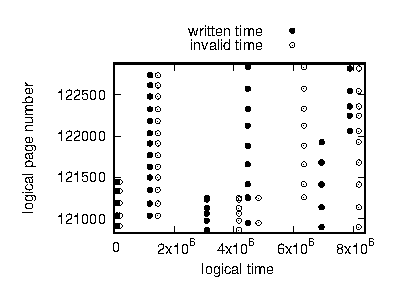
\includegraphics[width=0.9\linewidth]{figure/chunklifetime} % data from 1/02271857 - 59 chunk 
	\caption{The various lifetime of data of append-only workload with in a chunk}
	\label{fig:chunklifetime}
\end{figure}

Summarizing existing studies, if we adopt automated stream management to the append-only workload,
we lose the lifetime information of the application. 



%\documentclass[onecolumn, 10pt]{IEEEtran}
%\linespread{2.4}

\documentclass[letterpaper, twocolumn, 10pt]{article}

\usepackage{usenix}
\usepackage{multirow}
\usepackage{comment}
\usepackage{epsfig}
%\usepackage{kotex}
%\usepackage{amsmath}
\usepackage{amssymb}
\usepackage{multirow}
\usepackage{url}
\usepackage{subfig}
\usepackage{color}
\usepackage{xcolor}
\usepackage{cases}
\usepackage{graphicx}
%\usepackage{float}
%\usepackage{caption}
\DeclareCaptionType{copyrightbox}

\begin{document}

\title{
PCStream
%Improving Lifetime of SSD-based RAIDs using Dedup-assisted Partial Stripe Writes
}

%\numberofauthors{1}

\author{
Taejin Kim
}

\maketitle

\thispagestyle{empty}

\subsection*{Abstract}
TBD

\section{Introduction}
TBD

\section{Motivation}
TBD

\section{PCStream}
TBD

\section{Experimental Results}
TBD

\section{Conclusion}
TBD


\end{document}

\vspace{-10pt}
\section{Experimental Results}
\vspace{-5pt}

\begin{figure*}[t]
	\centering
	\vspace{-3pt}
	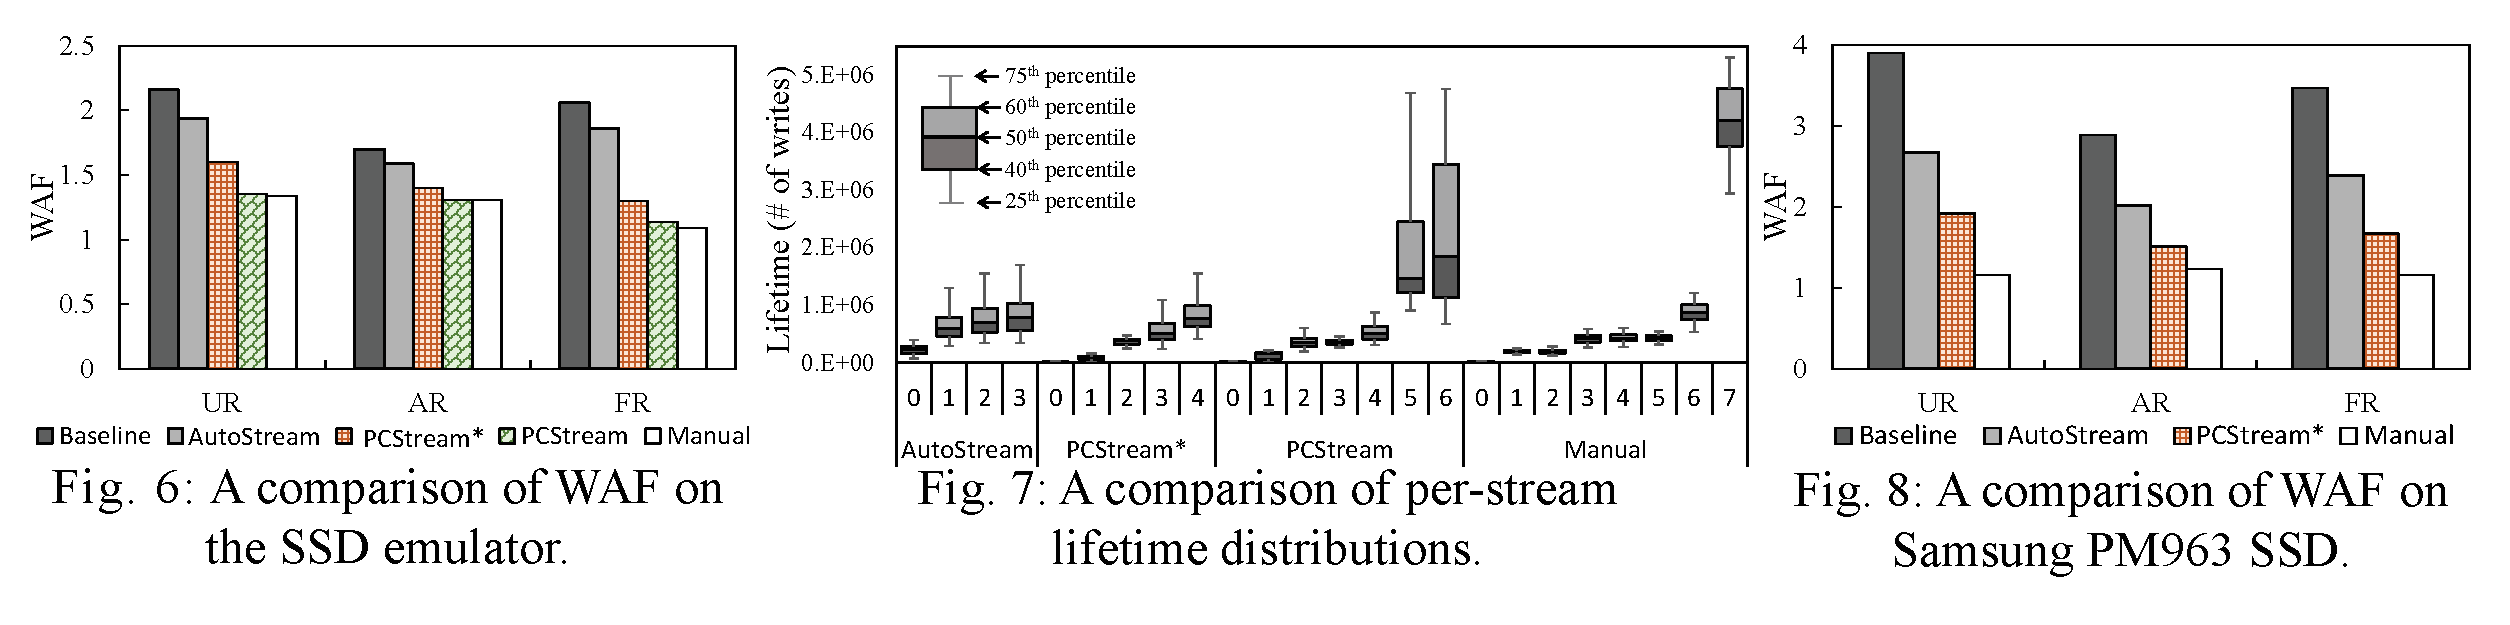
\includegraphics[width=1\textwidth]{figure/expfig}
%	\subfloat[\scriptsize{A comparison of WAF on the SSD emulator}.]{\label{fig:result_emul}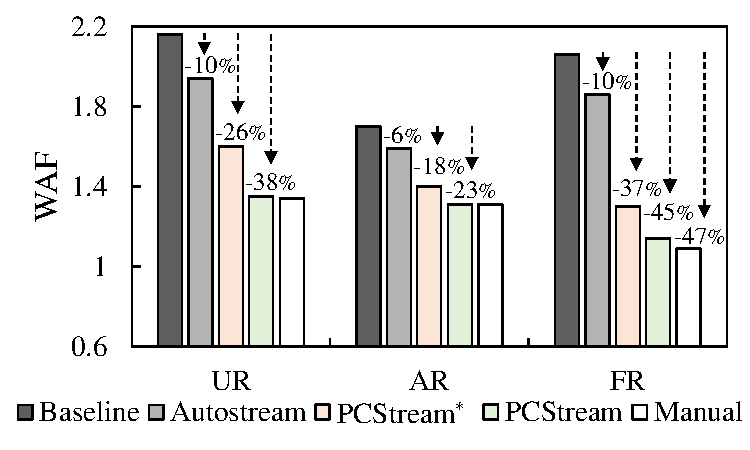
\includegraphics[width=0.33\textwidth]{figure/result_emul}}
%	\subfloat[\scriptsize{A comparison of WAF on PM963}.]{\label{fig:result_ssd}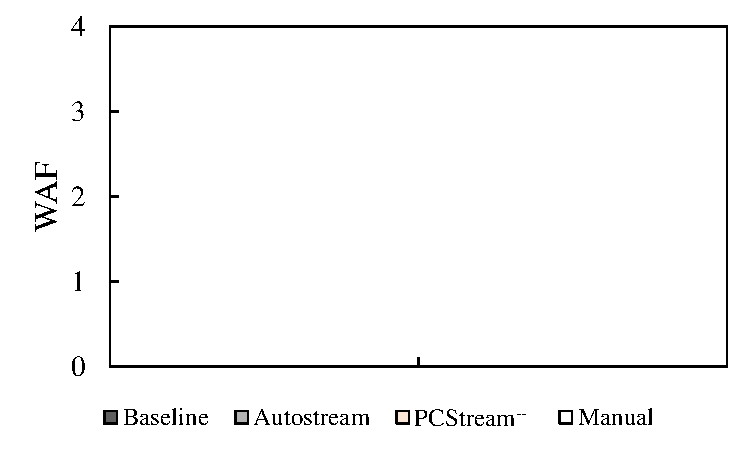
\includegraphics[width=0.33\textwidth]{figure/result_ssd}}
%	\subfloat[\scriptsize{A lifetime comparison of each stream}.]{\label{fig:streamlifetime}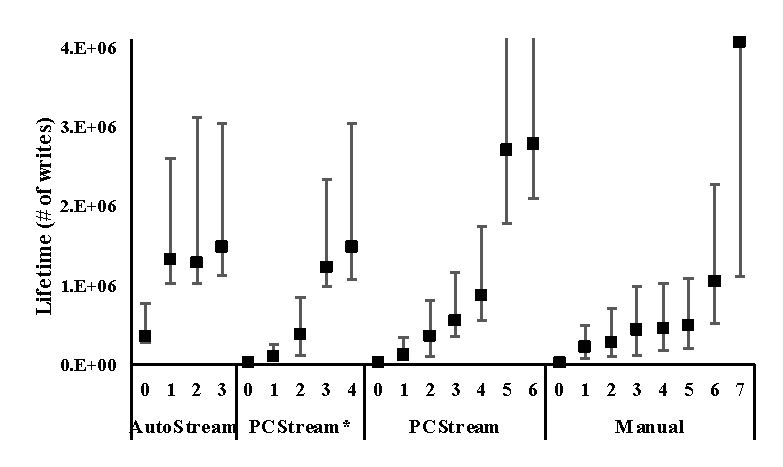
\includegraphics[width=0.33\textwidth]{figure/streamlifetime}}
%	\vspace{-10pt}
%	\caption{The WAF comparison on the emulator.}
	\label{fig:exp}
	\vspace{-35pt}
\end{figure*}

For our experiments, we have implemented \textsf{\small PCStream} in the Linux kernel
4.5.  For an objective evaluation, we compared \textsf{\small PCStream} with three
existing schemes: \textsf{\small Baseline}, \textsf{\small Manual}~\cite{MultiStream}, and
\textsf{\small AutoStream}~\cite{AutoStream}.  \textsf{\small Baseline} stands for a legacy
SSD that does not support a multi-stream feature. \textsf{\small Manual} is a RocksDB
implementation which is manually optimized for multi-streamed SSDs.
\textsf{\small AutoStream} is an LBA-based data separation technique which is
implemented at the block driver layer. To understand the impact of the
two-phase assignment, in addition, we compared \textsf{\small PCStream} with
\textsf{\small PCStream$^{*}$} which excluded the two-phase assignment feature.

For benchmarks, we have used three scenarios of \texttt{db\_bench} of RocksDB:
Update-Random (\texttt{UR}), Append-Random (\texttt{AR}), and Fill-Random
(\texttt{FR}) scenarios.  For key-value pairs already stored in the SSD,
\texttt{UR} updates values for random keys, creating many
read-modify-writes in the SSD.  \texttt{AR} is similar to \texttt{UR}, except
that it performs the update of values for growing keys. \texttt{FR} writes
key-value pairs to the SSD in a random key order.

\vspace{-10pt}
\subsection{Experiments with an SSD emulator}
\vspace{-2pt}

\begin{comment}
\begin{figure}[t]
	\centering
	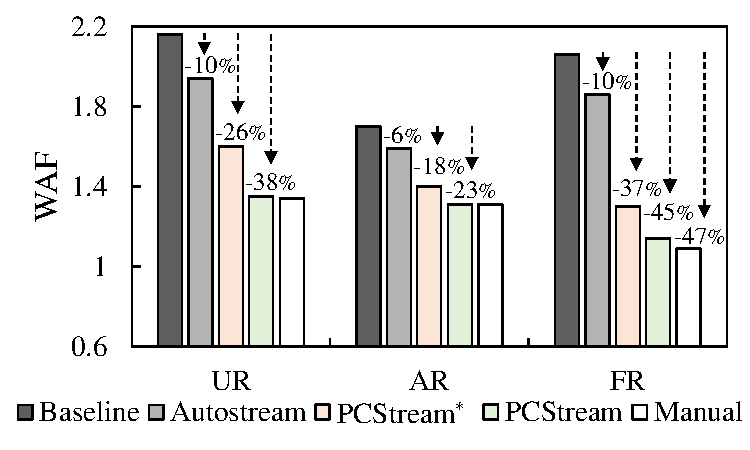
\includegraphics[width=0.8\linewidth]{figure/result_emul}
	\vspace{-10pt}
%	\caption{The WAF comparison on the emulator.}
	\caption{A comparison of WAF on the SSD emulator.}
	\label{fig:result_emul}
	\vspace{-15pt}
\end{figure}

 \begin{figure}[b]
	\centering
	\vspace{-15pt}
	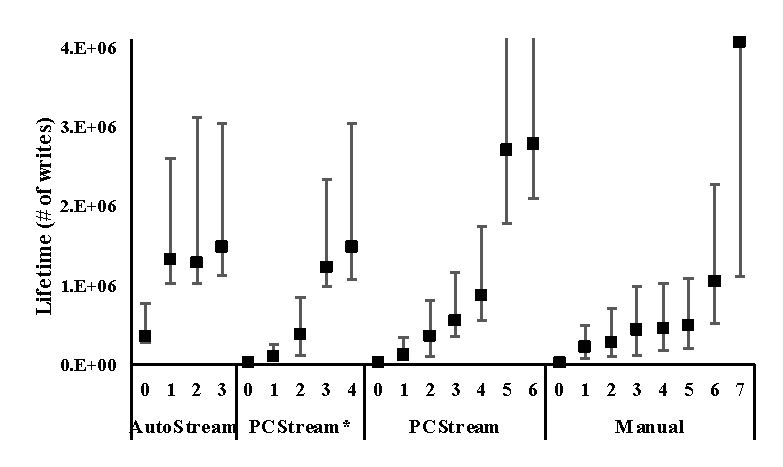
\includegraphics[width=1\linewidth]{figure/streamlifetime}
	\vspace{-20pt}
%	\caption{The WAF comparison on the emulator.}
	\caption{A lifetime comparison of each stream}
	\label{fig:streamlifetime}
\end{figure}

\begin{figure}[t]
	\centering
	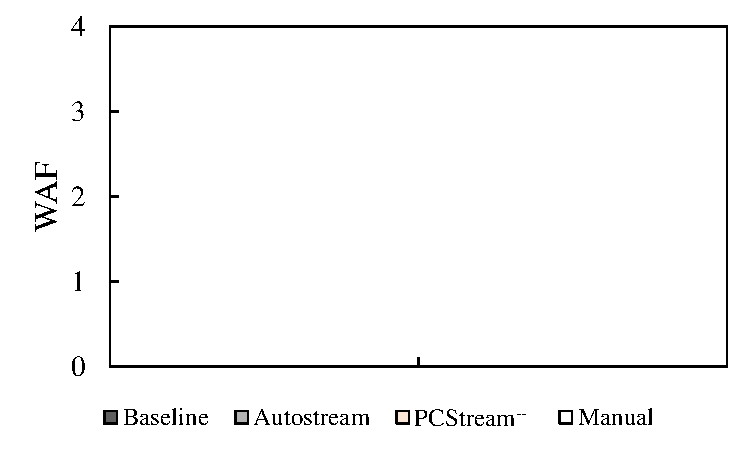
\includegraphics[width=0.8\linewidth]{figure/result_ssd}
	\vspace{-10pt}
	\caption{A comparison of WAF on PM963.}
	\label{fig:result_SSD}
	\vspace{-15pt}
\end{figure}
\end{comment}


We carried out a set of experiments using an SSD emulator which is based on the
open flash development platform~\cite{AMF}.  
%The SSD emulator emulates the behaviors of an SSD using host DRAM in the kernel level. Thus, it not only allows us to easily add new features, but enables to analyze detailed internal activities of an SSD. 
In the SSD emulator, the internal workings of an SSD are simulated using the host's DRAM memory in the kernel level. 
For our evaluations, we extended the SSD emulator to support a multi-streamed feature %.
(up to 8 streams). %shane part
Furthermore, we enhanced the garbage collection module of the SSD firmware to support the two-phase stream management technique. 
%We assume that the SSD emulator supports up to 8 streams (as with Samsung PM963 which was used in our experiments). %shane part
%We enhanced the original emulator so that it supported a multi-streamed feature as well as the two-phase stream assignment.  The number of streams supported by the emulator was 8.  
The SSD emulator provided 12 GB capacity with 4 channels and 4 ways, and there were 8192 flash blocks, each of which was composed of 384 4-KB pages.  


We compared WAF of the existing techniques with \textsf{\small PCStream} for the three
scenarios, and the result is shown in Fig. 6.  
\textsf{\small PCStream} was quite effective in reducing WAF, 
thus achieving an equivalent level of the WAF reduction as in \textsf{\small Manual}.  
For example, both \textsf{\small PCStream} and \textsf{\small Manual} reduced WAF by 38\% over \textsf{\small Baseline} for the \texttt{UR} case. 
%Compared with \textsf{\small AutoStream}, \textsf{\small PCStream} was more effective, reducing WAF more by 35\% on average.  
\textsf{\small PCStream} outperformed \textsf{\small AutoStream} by reducing WAF by 35\% on average.
Fig. 6 also indicates that the two-phase stream assignment technique is effective.  
\textsf{\small PCStream} outperformed \textsf{\small PCStream$^{*}$} by 12\% on average in the WAF reduction.
%As shown in Fig. 6, \textsf{\small PCStream$^*$} reduced WAF by up to 30\% over \textsf{\small AutoStream}.  
%The result shows that separating short-lived data (e.g., log and flush) from long-lived one (e.g., compaction) using PC was quite effective in reducing WAF.  Moreover, \textsf{\small PCStream} even showed similar WAF to \textsf{\small Manual}, reducing it by up to 38\% over \textsf{\small AutoStream}.  
This additional gain of \textsf{\small PCStream} over \textsf{\small PCStream$^{*}$} came from isolating long- and short-lived data in separate blocks 
%through the two-phase assignment at the SSD even if they belonged to the same compaction PC.
%by moving the long-lived data of the compaction-activity PC to substreams during GC at the SSD.
by moving the long-lived data to substreams during GC at the SSD.


In order to better understand how \textsf{\small PCStream} achieved a high reduction in WAF, 
we measured per-stream lifetime distributions under each technique for the \texttt{UR} scenario.
Fig. 7 shows a box plot of data lifetimes from the 25th percentile to the 75th percentile.
%In order to analyze the improvement made by \textsf{\small PCStream}, 
%we measured the data lifetime of each stream for the {\tt UR} scenario.
%Fig. 7 shows average, 75p, and 25p of data liftime for each stream.
As shown in Fig. 7, 
streams in \textsf{\small PCStream} are divided into two groups, 
$G1$ = $\{$0, 1, 2, 3, 4$\}$ and $G2$ = $\{$5, 6$\}$, 
where $G1$ includes streams with short lifetimes and small variances %(i.e., streams 0, 1, 2, 3, and 4) 
and $G2$ includes streams with large lifetimes and large variances.  %(i.e., streams 5 and 6).  
%By preventing $G1$ and $G2$ from mixing in the same block, \textsf{\small PCStream} can reduce the GC overhead.  
Since the GC copy cost is affected by how data in $G1$ and $G2$ are mixed into the same block, 
\textsf{\small PCStream} can significantly reduce the GC overhead 
by avoiding such data mixtures in the same block by separating $G1$ and $G2$ into different streams. 
On the other hand, in \textsf{\small AutoStream}, 
three streams (i.e., streams 1, 2, and 3) show similar lifetime distributions with large variances 
without a distinct data separation pattern.
%Unlike \textsf{\small PCStream} and \textsf{\small Manual}, \textsf{\small AutoStream} does not show that 
%their streams are divided based on data lifetimes.  
%Such stream allocation is not effective in reducing the GC copy cost. 
%, thus not effectively taking full advantage of streams.
%data lifetimes of stream 0 to 5 in \textsf{\small Manual} are gathered in a narrow range so data lifetime in the same is quite similar.
%However, data lifetime of streams in \textsf{\small AutoStream} shows relatively large difference
%\textsf{\small AutoStream} does not notice when long-lived data is written to the hot stream.
%On the other hand, \textsf{\small PCStream$^*$} can identify short-lived data from 
%several dominant I/O activities as mentioned in section 2, for example, stream 0 and 1 in the Fig. 7.
%\textsf{\small PCStream} can further separate long-lived data of several streams (e.g., stream 3 and 4)
%by moving their data to substreams (e.g., stream 5 and 6, respectively). 
In Fig. 7, we can also observe the effect of substreams.  
Streams 3 and 4 of \textsf{\small PCStream$^{*}$}, 
which have large variances in lifetimes, are split into two substreams 5 and 6 in \textsf{\small PCStream}.
This split reduces variances of streams 3 and 4, thus reducing the GC copy cost.  %improving WAF. 

\vspace{-8pt}
\subsection{Experiments with a real-world SSD}
\vspace{-2pt}

In order to evaluate the effect of \textsf{\small PCStream} in a real SSD,  
%In order to confirm the feasibility of \textsf{\small PCStream}, 
we have
conducted experiments using Samsung's PM963 480GB SSD that supports 8 streams.
Since it was impossible to implement the two-phase stream assignment in the
commercial SSD firmware, we evaluated \textsf{\small PCStream$^*$} only.  To warm up the
SSD before running benchmarks, we filled up 90\% of the SSD capacity with valid
data.
As illustrated in Fig. 8, \textsf{\small PCStream$^*$} reduced WAF by
28\% over \textsf{\small AutoStream} on average.  
%There were large WAF gaps between \textsf{\small PCStream$^{*}$} and the manually optimized case.  If the substream was properly supported during GC, we believe that \textsf{\small PCStream} could show similar WAF values as \textsf{\small Manual}.  
Note that although \textsf{\small PCStream$^*$} still outperformed \textsf{\small AutoStream} in PM963, 
but a performance gap was smaller over that
in the emulated SSD environment.  It was difficult to pinpoint why
\textsf{\small AutoStream} worked better in PM963 over in the emulated SSD, but we
suspect that some internal features of PM963 (such as a large block size or some implementation details of streams) %might be related. 
might have affected the performance of \textsf{\small AutoStream}.


\vspace{-13pt}
\section{Conclusions}
%\vspace{-5pt}
We have presented a new stream management technique, \textsf{\small PCStream}, for multi-streamed SSDs.  
Unlike existing stream management techniques, \textsf{\small PCStream} fully automates 
the process of mapping data to a stream based on PCs, 
which work well for append-only workloads as well as update workloads.  
By exploiting an observation that most PCs are distinguishable from each other 
in their lifetime characteristics, \textsf{\small PCStream} allocates each PC to a different stream.  
When a PC has a large variance in their lifetimes, \textsf{\small PCStream} refines its stream allocation 
during garbage collection and moves the long-lived data of the current stream to its substream.  
%Our experimental results show that \textsf{\small PCStream} can reduce WAF by up to 38\% over the existing
Our experimental results show that \textsf{\small PCStream} can reduce the average WAF by 35\% over the existing %shane part
automatic technique.

The current version of \textsf{\small PCStream} can be extended in several directions.  
For example, we plan to optimize the PC clustering method so that
multiple PCs can be better clustered when the number of PCs significantly
outnumbers the number of streams.  
%For example, \textsf{\small PCStream} should be improved in its PC clustering method 
%so that it can work effectively even when there are more PCs than the number of streams.  
%We also plan to evaluate \textsf{\small PCStream} (not \textsf{\small PCStream}$^{--}$) on real SSDs 
%by implementing the two-phase stream assignment algorithm inside an FTL.


\bibliographystyle{abbrv}
\bibliography{sigproc}
\begin{thebibliography}{00}

\bibitem{T10}
TBD

\bibitem{MultiStream}
J.-U. Kang, J. Hyun, H. Maeng, and S. Cho. The Multi-streamed Solid-State Drive.
In \textit{Proceedings of the 6th Workshop on Hot Topics in Storage and File Systems (HotStorage'14)}, 2014.


\bibitem{FStream}
E. Rho, K. Joshi, S.-U. Shin, N.J. Shetty, J.-Y. Hwang, S. Cho. and D.DG. Lee. 
FStream: Managing Flash Streams in the File System.
In \textit{Proceedings of the 16th USENIX Conference on File and Storage Technologies (FAST'18)}, 2018.

\bibitem{AutoStream}
J. Yang, R. Pandurangan, C. Chio, and V. Balakrishnan.
AutoStream: Automatic Stream Management for Multi-streamed SSDs.
In \textit{Proceedings of 10th ACM International Systems and Storage Conference (SYSTOR'17)}, 2017.

\bibitem{Level}
F. Yang, D. Dou, S. Chen, M. Hou, J.-U. Kang, and S. Cho.
Optimizing NoSQL DB on Flash: A Case Study of RocksDB.
In \textit{Proceedings of IEEE 15th International Conference on Scalable Computing
and Communications}. 2015.

\bibitem{PCHa}
K. Ha, and J. Kim.
A Program Context-Aware Data Separation Technique for Reducing Garbage Collection Overhead in NAND Flash Memory.
In \textit{Proceedings of International Workshop on Storage Network Architecture 
and Parallel I/Os (SNAPI'11)}, 2011.

\bibitem{RocksDB}
Facebook, https://github.com/facebook/rocksdb

\bibitem{Cassandra}
Apache Cassandra, http://cassandra.apache.org

\bibitem{PC}
F. Zhou, J.R. von Behren, and E.A. Brewer.
Amp: Program Context Specific Buffer Caching.
In \textit{Proceedings of USENIX Annual Technical Conference (ATC'05)}, 2005.

\bibitem{TRIM}
TBD.

\bibitem{LSM}
P. ONeil, E. Cheng, D. Gawlick, and E. ONeil.
The Log-Structured Merge-Tree (LSM-Tree).
In \textit{Acta Informatica, v.33, n.4, p.351-385}, 1996

\bibitem{GCC}
R.M. Stallman, and GCC Developer Community.
Using the GNU Compiler Collection for GCC version 7.3.0.
https://gcc.gnu.org/onlinedocs/gcc-7.3.0/gcc.pdf. 2018.

\bibitem{AMF}
S. Lee, M. Liu, S. Jun, S. Xu, J. Kim, and Arvind.
Application-Managed Flash.
In \textit{Proceedings of 14th USENIX Conference on File and Storage
Technologies (FAST'16)}, 2016.

\end{thebibliography}

\end{document}
